\documentclass{article}
\usepackage{titling}
\usepackage{lipsum}
\usepackage{amsmath}
\usepackage{listings}
\usepackage{graphicx}
\usepackage{subcaption}
\usepackage{pgfplots}
\usepackage[margin=1in]{geometry}
\usepgfplotslibrary{statistics}



\begin{document}
\noindent
\begin{minipage}[t]{0.6\textwidth}
    \begin{flushleft}
        \LARGE\textbf{Math 343 - Lab 5} \\
        \vspace{6pt} % add 6pt of vertical space
        \hrule width 10cm
        \vspace{12pt}
        \large\textbf{Preston Duffield} \\
        \large Western Washington University \\
        \today
        % April 18, 2023
        \vspace{24pt}
    \end{flushleft}
\end{minipage}

\section*{Question 1}
\subsection*{a)}
To estimate value of $(\tau \beta)_{22}$, first must observe that
$\bar{y}_{2 2 \cdot} = \frac{100 + 85.9}{2} = 92.95$.
$\bar{y}_{2 \cdot \cdot} = 85.9$.
$\bar{y}_{\cdot 2 \cdot} = 100$.
$\bar{y}_{\cdot \cdot \cdot} = \frac{100 + 79.2 + 85.9 + 83.9}{4} = 87.25$. \\

Therfore: $(\hat{\tau \beta})_{22} = 92.95 - 85.9 - 100 + 87.25 = -5.7$
\subsection*{b)}
First we note the following: \\
$\hat{\mu}_{11} = 83.9$ \\
$\hat{\mu}_{12} = 85.9$ \\
$\hat{\mu}_{22} = 100$ \\
$\hat{\mu}_{21} = 79.2$ \\
The main effect of source of protien (A) is: \\
$\frac{79.2 + 100}{2} - \frac{83.9 + 85.9}{2} = 4.7$ \\

The main effect of amount of protien (B) is: \\
$\frac{85.9 + 100}{2} - \frac{83.9 + 100}{2} = 1$ \\

The interaction effect of the two sources is: \\
$\frac{100 + 83.9}{2} - \frac{79.2 + 85.9}{2} = 9.4$ \\
\subsection*{c)}
\begin{figure}[h]
    \centering
    \includegraphics[width=0.5\textwidth]{./images/1_c.png}
    \caption{The ANOVA table from Minitab.}
    \label{fig:1_c}
  \end{figure}

$\alpha = 0.10$, for each following test. \\
Test of Significance of Main Effects of Factor A:
$H_0$: $\tau_1 = \tau_2 = 0$ \\
$H_a$: At least one $\tau_i$ is different.\\

Since the p-value $= 0.327 > \alpha$, we can conlcude the following.
There is not enough statistical evidence to support the hypothesis
that at least one $\tau_i$ is different.
\\
Test of Significance of Main Effects of Factor B:
$H_0$: $\beta_1 = \beta_2 = 0$ \\
$H_a$: At least one $\beta_i$ is different.\\

Since the p-value $= 0.021 < \alpha$, we can conlcude the following.
There is enough statistical evidence to support the hypothesis
that at least one $\beta_i$ is different.
\\
Test of Significance of Main Effects of Factor B:
$H_0$: $(\tau \beta)_{11} = (\tau \beta)_{12} = (\tau \beta)_{22} = (\tau \beta)_{21} = 0$ \\
$H_a$: At least one $\tau \beta)_{ij}$ is different.\\

Since the p-value $= 0.054 < \alpha$, we can conlcude the following.
There is enough statistical evidence to support the hypothesis
that at least one $\tau \beta)_{ij}$ is different.


\subsection*{d)}
\begin{figure}[h]
    \centering
    \includegraphics[width=0.5\textwidth]{./images/1_d.png}
    \caption{Interaction plot from Minitab.}
    \label{fig:1_d}
  \end{figure}
\subsubsection*{i.}
Yes. Since the lines are not relatively parallel there appears to be interaction.
\subsubsection*{ii.}
Effect of source of protein from graph $\sim 4.5$. This does support my previous answer.
\subsubsection*{iii.}
Effect of source of protein at the “low” level $\sim 4.7$. This does support my previous answer.
\subsubsection*{iv.}
I would choose source: beef, and Level: high to increase the weight gain in rats.
\subsection*{e)}
The confidence interval formula is:
$\bar{y}_{i \cdot \cdot} - \bar{y}_{i` \cdot \cdot} \pm q_{\alpha, a, df_{error}}\sqrt{\frac{MSE}{b \cdot n}}$

The 95\% C.I. for the mean weight gain corresponding to high protien diet is:
$\bar{y}_{2 \cdot \cdot} - \bar{y}_{1 \cdot \cdot} \pm q_{.05, 2, 1}\sqrt{\frac{MSE}{2 \cdot 10}}$ \\
$100 - 85.9 \pm 3.67\sqrt{\frac{223.6}{20}}$
$14.1 \pm 12.27$
\section*{Question 2}
\subsection*{a)}
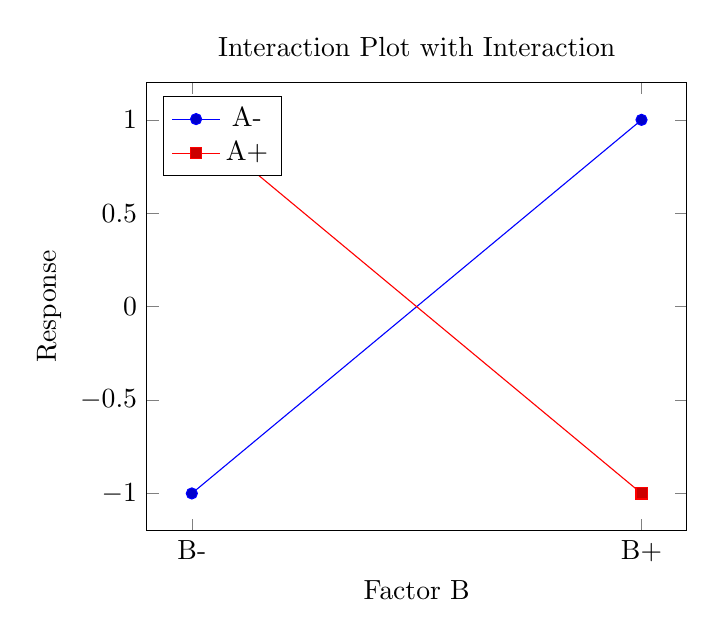
\begin{tikzpicture}
    \begin{axis}[
        title={Interaction Plot with Interaction},
        xlabel={Factor B},
        ylabel={Response},
        symbolic x coords={B-, B+},
        xtick=data,
        legend pos=north west
    ]
    \addplot coordinates {(B-, -1) (B+, 1)};
    \addplot coordinates {(B-, 1) (B+, -1)};
    \legend{A-,A+}
    \end{axis}
    \end{tikzpicture}
\subsection*{b)}
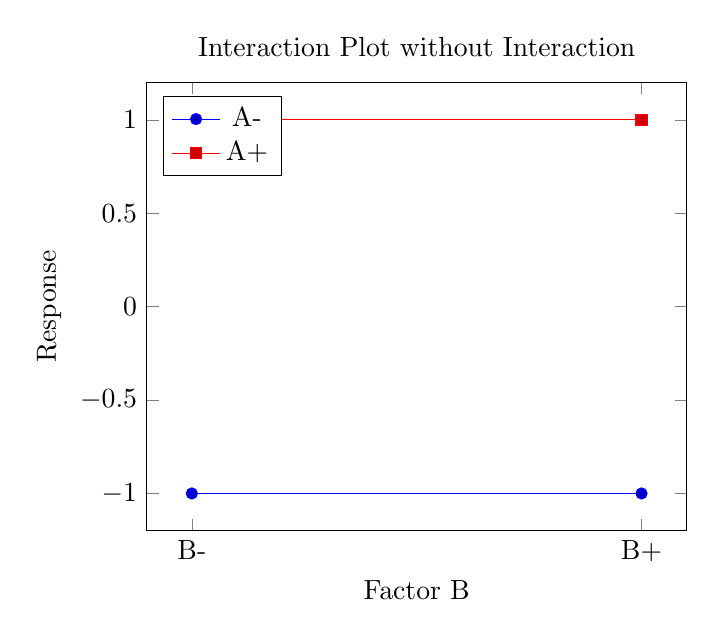
\begin{tikzpicture}
    \begin{axis}[
        title={Interaction Plot without Interaction},
        xlabel={Factor B},
        ylabel={Response},
        symbolic x coords={B-, B+},
        xtick=data,
        legend pos=north west
    ]
    \addplot coordinates {(B-, -1) (B+, -1)};
    \addplot coordinates {(B-, 1) (B+, 1)};
    \legend{A-,A+}
    \end{axis}
    \end{tikzpicture}


\end{document}
